\documentclass[xcolor={dvipsnames}]{beamer}

\usetheme{Malmoe}
\usecolortheme{seagull}
\usepackage[]{natbib}
\usepackage{textpos}
\usepackage{amsmath, amssymb, bm}
\usepackage{multirow}
\usepackage{framed}
\usepackage{schemata}
\setbeamertemplate{navigation symbols}{}
\usepackage[english]{babel}
\usepackage{animate}
\usepackage{graphics}
\usepackage{fontawesome}


\definecolor{lightblue}{rgb}{0.145,0.6666,1} % Defines the color used for content box headers
\definecolor{Red}{rgb}{0.9,0.15,0}
\definecolor{Blue}{RGB}{55,126,184}
\definecolor{Green}{RGB}{77,175,74}
\definecolor{White}{RGB}{255,255,255}
\definecolor{Lightgray}{rgb}{0.86,0.86,0.86}

\setbeamertemplate{footline}
{
	\leavevmode%
	\hbox{%
		\begin{beamercolorbox}[wd=.50\paperwidth,ht=2.25ex,dp=1ex,center]{author in head/foot}%
			\usebeamerfont{author in head/foot}\insertshortauthor%% \beamer@ifempty{\insertshortinstitute}{}{(\insertshortinstitute)}
		\end{beamercolorbox}%
%		\hskip2pt%
		\begin{beamercolorbox}[wd=.50\paperwidth,ht=2.25ex,dp=1ex,center]{title in head/foot}%
			\usebeamerfont{title in head/foot}\insertshorttitle~~~~~~~~~~~~~~~~~~~~~~~~~~\insertframenumber
		\end{beamercolorbox}%
	}%
	\vskip0pt%
}
\makeatother

\title[Inequality and Uncertainty in Length of Life]{}

\subtitle{\large{\textsc{Homicides increased life uncertainty and inequality of lifespans in Mexico, 2005-2015}}\\$\,$\\}


\author[Aburto \& Beltr\'an-S\'anchez 2018]
{
	\vspace{-0.5cm}
	\texorpdfstring{
		\begin{columns}
			\column{.9\linewidth}
			\centering
			\normalsize{Jos\'{e} Manuel Aburto \& Hiram Beltr\'an-S\'anchez}\\
			$\,$\\
			
\includegraphics[scale=0.2]{Figures/SDU_Logo.jpg}\\     
				\vspace{0.5cm}
						\includegraphics[scale=0.2]{Figures/MPIDR.PNG}   
		\end{columns}
	}
	{Jos\'{e} Manuel Aburto}
}

\date[]{October 2018}

\beamertemplatenavigationsymbolsempty
\begin{document}


\begin{frame}[plain]
	\titlepage
\end{frame}
%%%%%%%%%%%%%%%%%%%%%%%%%%%%%%%%%%%%%%%%%%%%%%%%%%%%%%%%%%%%%%%%%%%%%%%%%
%%%%%%%%%%%%%%%%%%%%%%%%%%%%%%%%%%%%%%%%%%%%%%%%%%%%%%%%%%%%%%%%%%%%%%%%%
\section{Introducci\'on}

%%%%%%%%%%%%%%%%%%%%%%%%%%%%%%%%%%%%%%%%%%%%%%%%%%%%%%%%%%%%%%%%%%%%%%%%%
\begin{frame}
\Large{
		\begin{itemize}
		
		\item<1-> La \textbf{violencia} es un problema prioritario de salud pública en América Latina
		
		\item<2-> En la actualidad AL tiene la \textbf{tasa de homicidios m\'as alta del mundo} (16.3 per 100,000).
		
        \item<3-> Pa\'ises del centro de la regi\'on han experimentado un \textbf{resurgimiento} de homicidios.
        
        \item<4-> \textbf{En M\'exico, la tasas se duplicaron entre 2007 y 2012} (9.3 $\longrightarrow$ 18.6).
		
		\end{itemize}
		
}

\end{frame}


\begin{frame}

\Large{
		\begin{itemize}
		    
		\item La esperanza de vida de hombres se estanc\'o en 2000-10 ($\backsim $72y)
		
				\end{itemize}
		
		\pause
				\begin{center}
		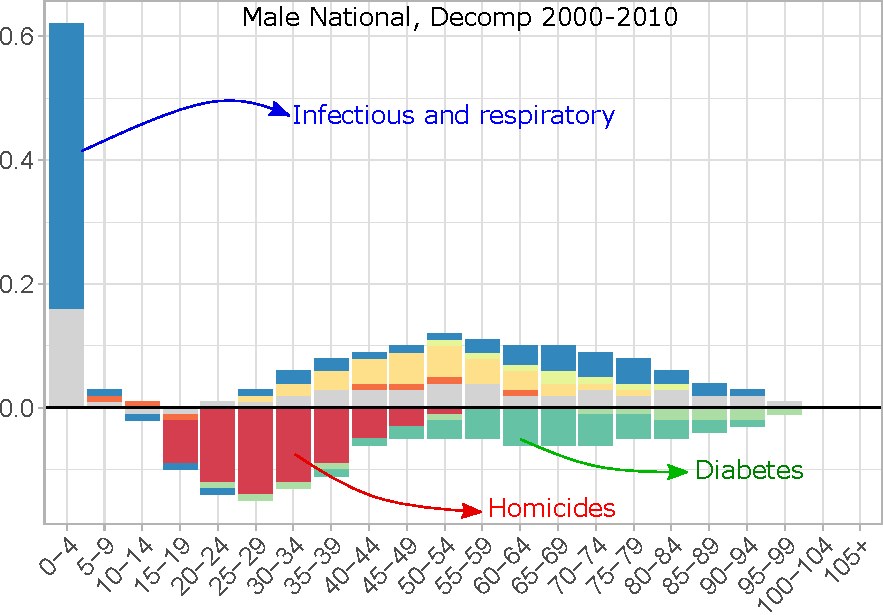
\includegraphics[scale=.55]{Figures/Fig_1}
				\end{center}
				

}
\end{frame}

\begin{frame}
\begin{center}
\Large{\textbf{Antes y despu\'es de la guerra contra las drogas y reforma en salud}}
\end{center}

\hspace*{-1cm}   
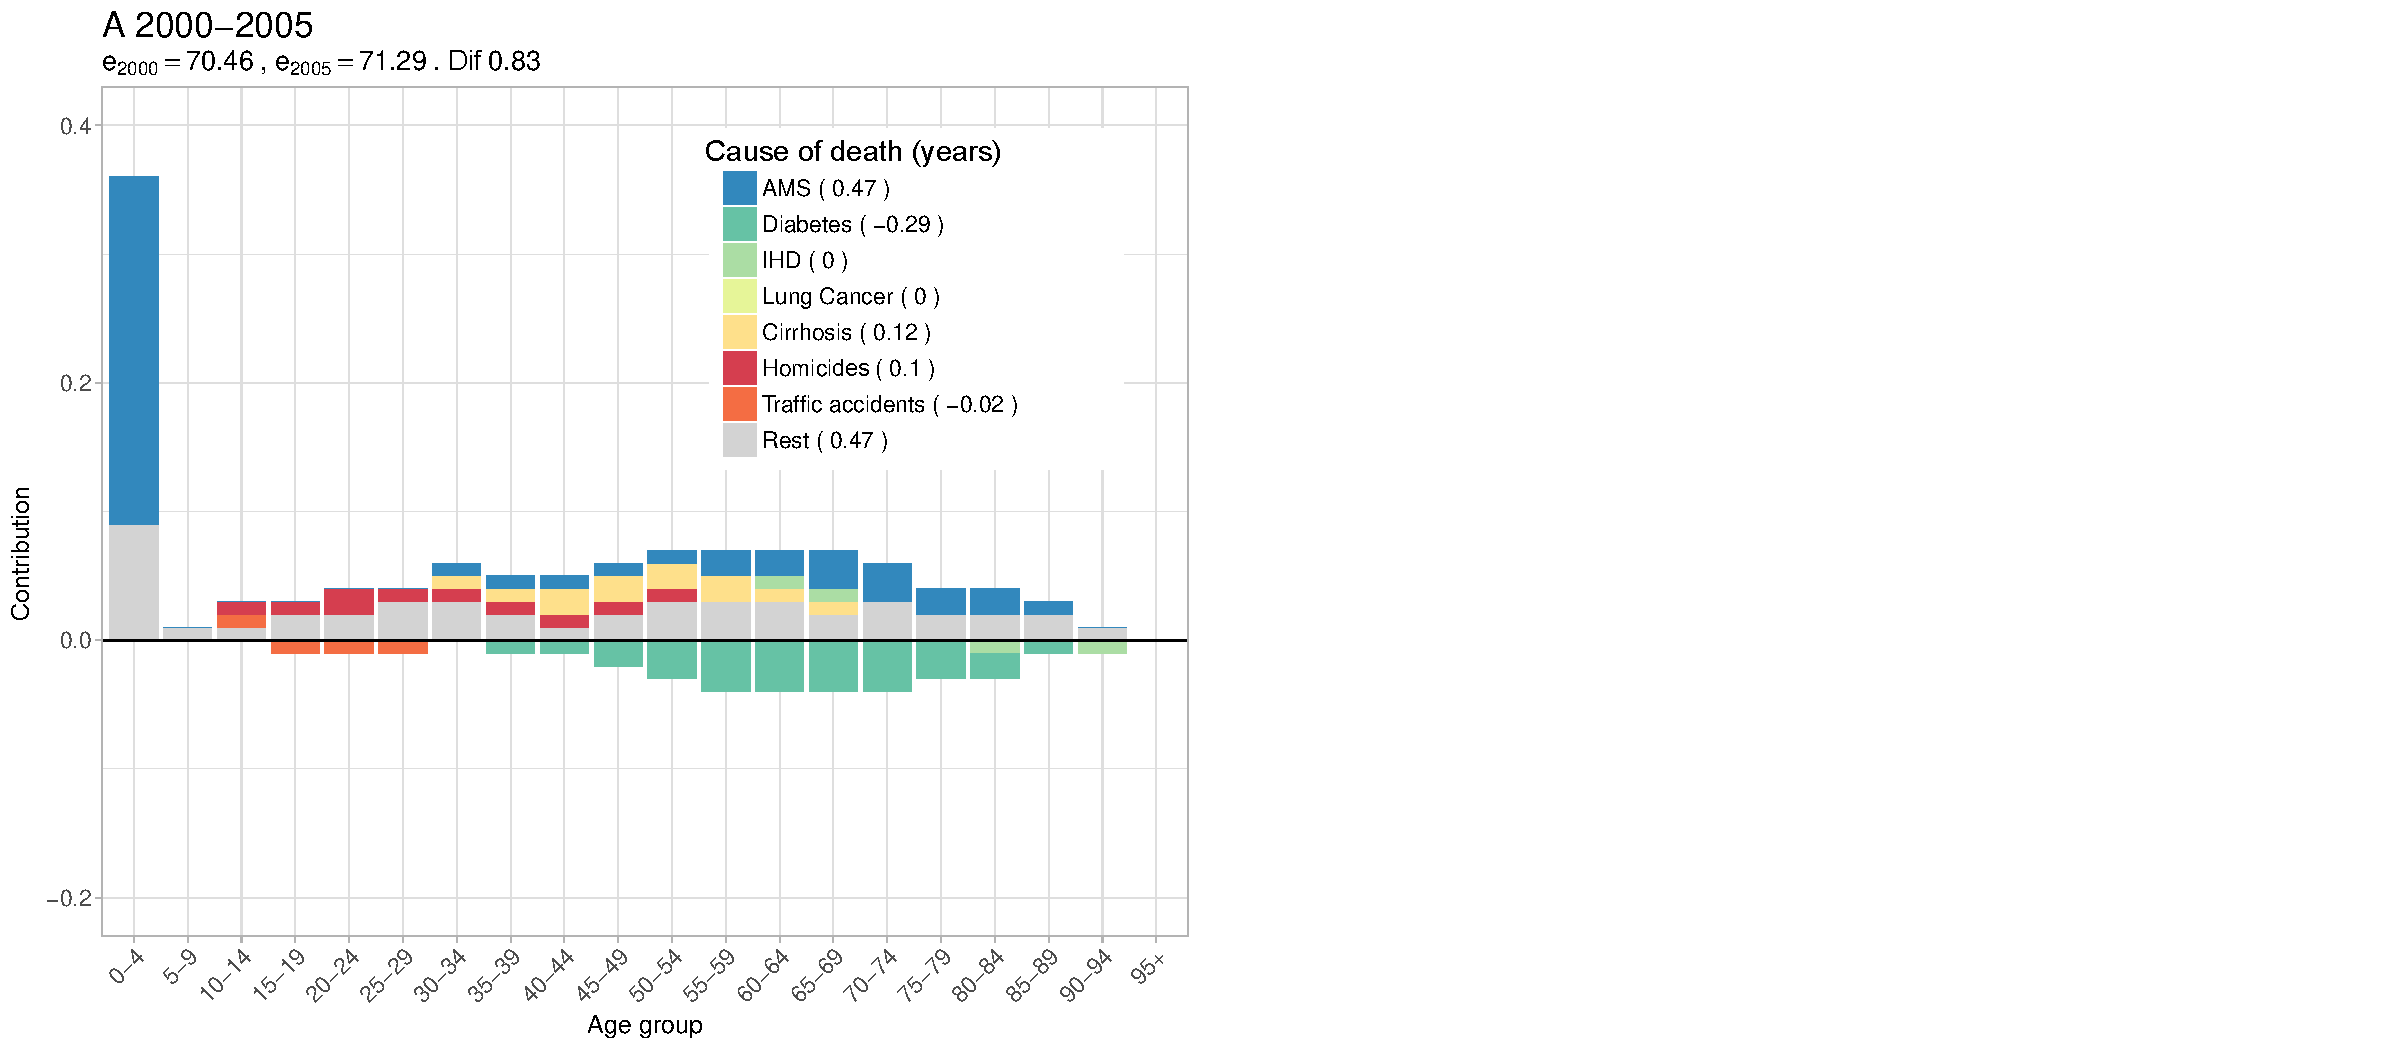
\includegraphics[scale=.31]{Figures/Fig2_1}

\end{frame}

\begin{frame}
\begin{center}
\Large{\textbf{Antes y despu\'es de la guerra contra las drogas y reforma en salud}}
\end{center}

\hspace*{-1cm}   
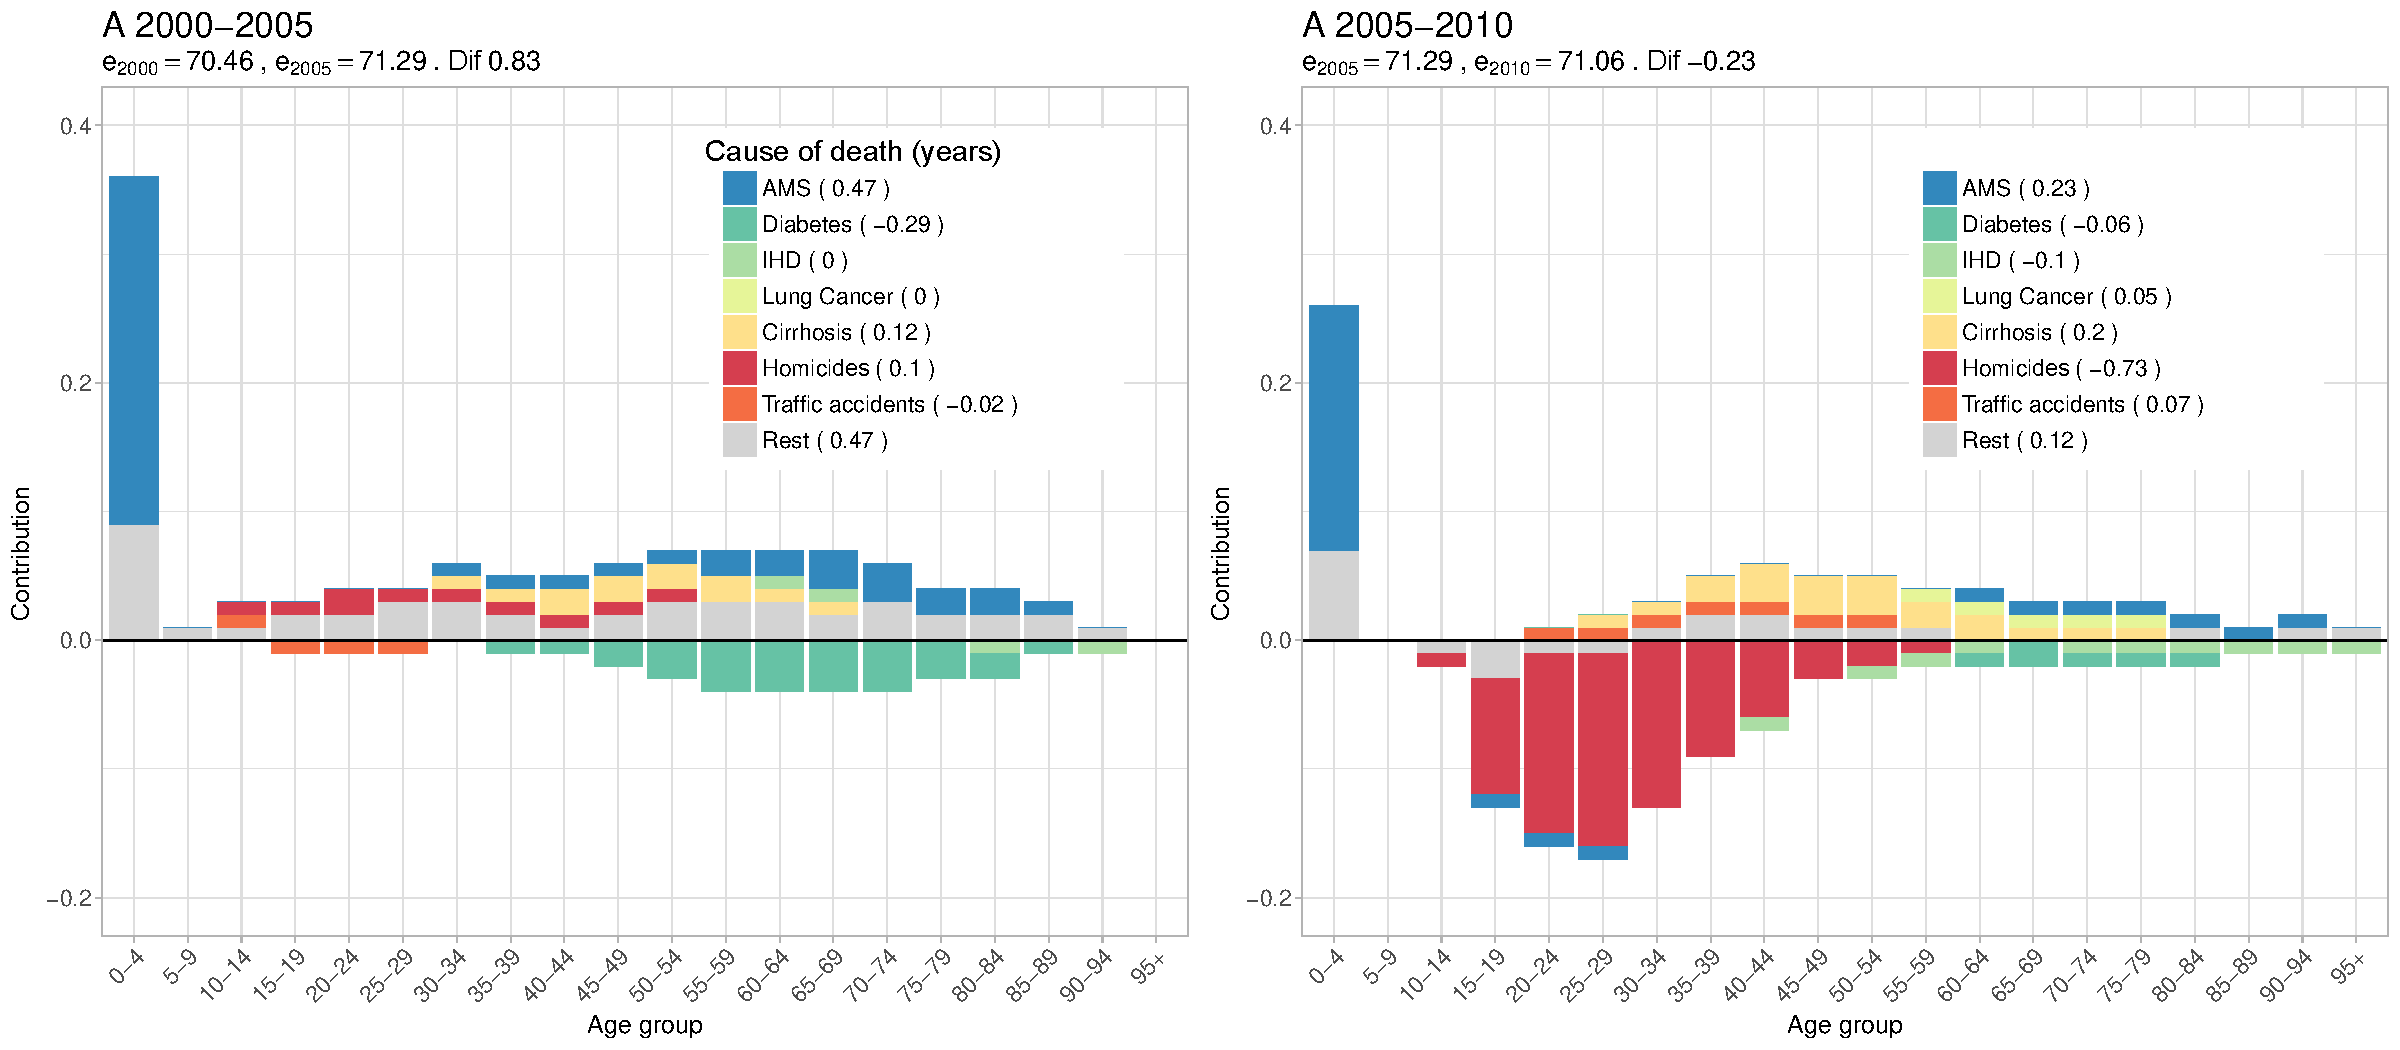
\includegraphics[scale=.31]{Figures/Fig2_2}

\end{frame}





\begin{frame}

				\begin{center}
		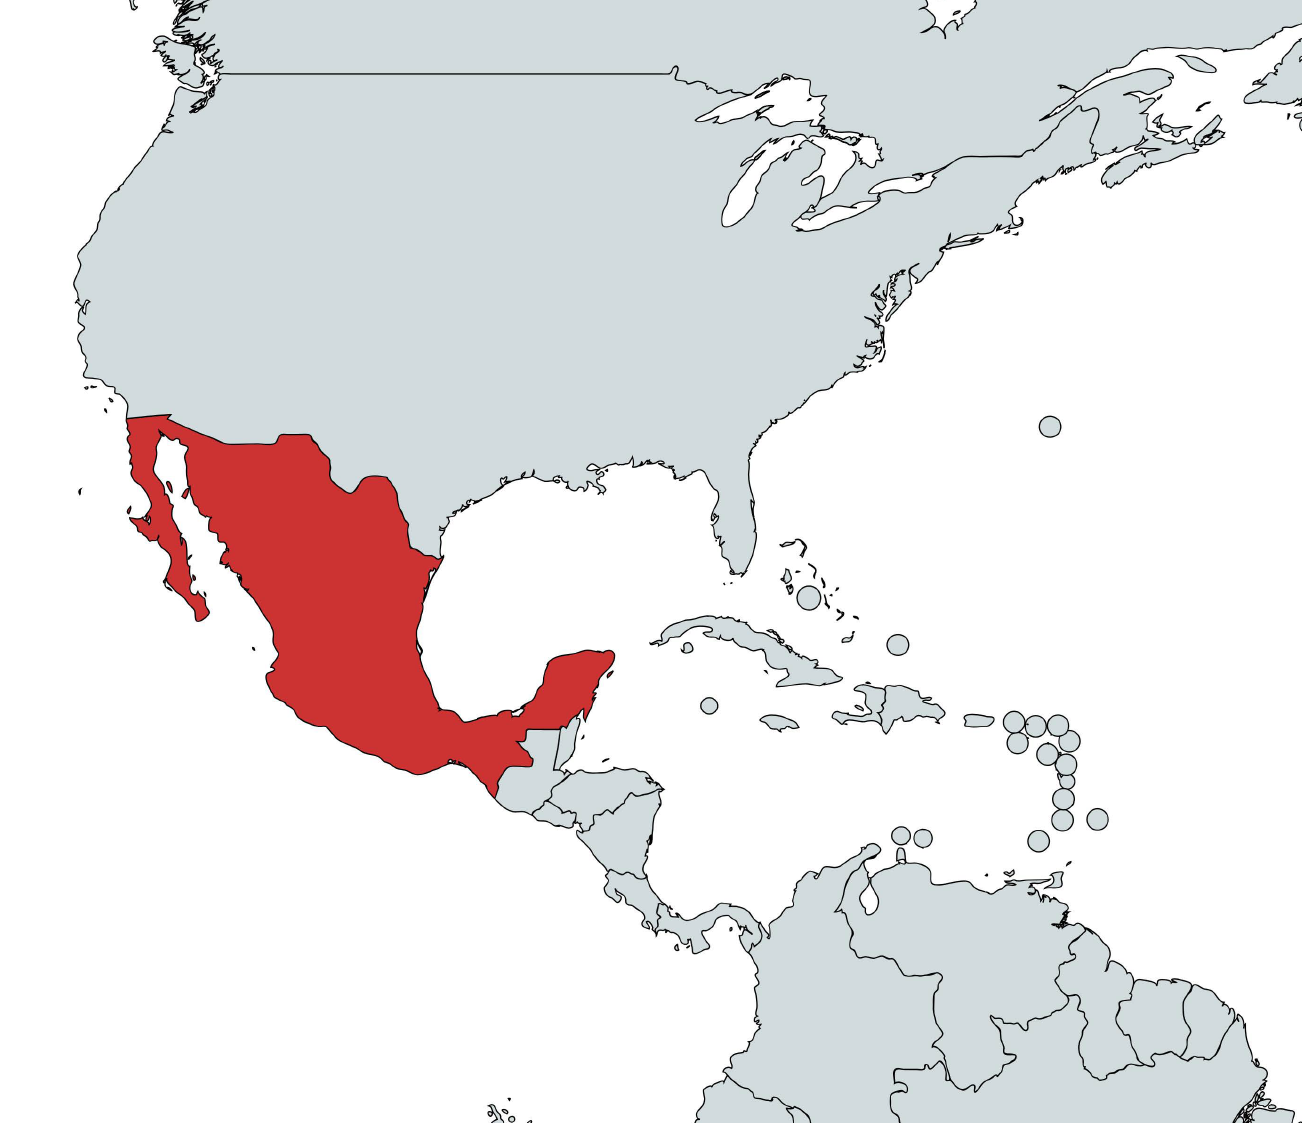
\includegraphics[scale=.3]{Figures/Mexico1}
				\end{center}
				
\end{frame}




\begin{frame}\frametitle{A nivel regional}


				\begin{center}
		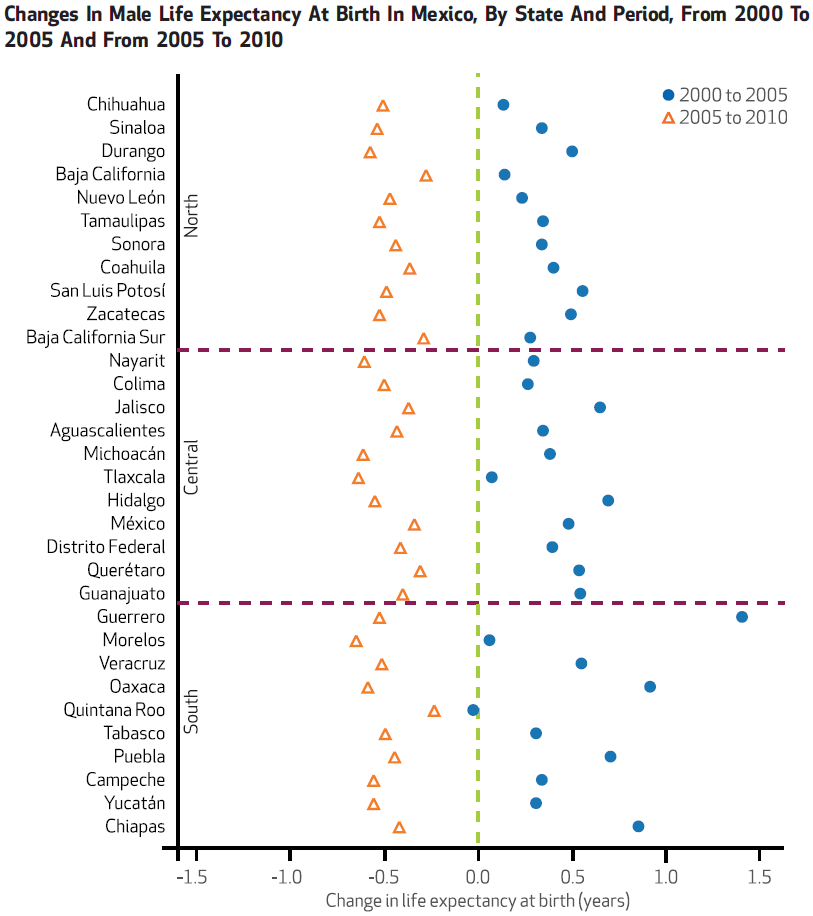
\includegraphics[scale=.37]{Figures/State_changes_e0}
				\end{center}
				
\end{frame}


\begin{frame}

\LARGE{
Ganancias en la esperanza de vida por causas susceptibles a servicio m\'edico

\begin{enumerate}
\item Enfermedades infecciosas
\item Enfermedades respiratorias
\item Condiciones del nacimiento
\item ...
\end{enumerate}

 \pause
\begin{center}
\textbf{Se revirtieron en la segunda mitad de 2000-10}
\end{center}				

}
\end{frame}


\begin{frame}
\Large{
Variaci\'on en la edad a la muerte (lifespan variation)
\pause
		\begin{itemize}
		
		\item \textbf{Decisiones de los individuos} (Esperanza de vida e incertidumbre). \pause

		\item \textbf{Periodos de incertidumbre o vulnerabilidad} llevan a cambios en la conducta. \pause
		
		\item Homicidios se concentran en \textbf{hombres j\'ovenes}. \pause
						
		\end{itemize}

}
\end{frame}

\section{M\'etodos}

\begin{frame}
\Large{
 Mortalidad \textbf{``Evitable/susceptible"}:
%An approach to approximate the impact of healthcare and other interventions, and to reveal potential areas of improvement. Based on causes that should not occur in the presence of effective and timely healthcare.
		\begin{enumerate}
		
		
\color{blue} 		\item Susceptibles a intervenciones m\'edicas 
\pause

\color{ForestGreen}		\item Diabetes
		
		\item Enfermedades isqu\'emicas del coraz\'on
		
		\item C\'ancer de pulm\'on.
		
		\item Cirrosis.
		
\pause
		
\color{red}		\item \textbf{Homicidios}
		
\color{yellow}		\item Accidentes de tr\'afico
		
		\pause
		
\color{gray}				\item Resto.

		
		\end{enumerate}			

}
\end{frame}


\begin{frame}

\Large{
\textbf{$e^{\dagger}_{15}\longrightarrow  $ }Esperanza de vida remanente al morir

\begin{itemize}
\item F\'acil  \textbf{interpretaci\'on}.
\pause
\item \textbf{Cuantifica} los efectos de la edad y causa de muerte.
\pause
\item Condicionamos a edad 15 para capturar el inicio de homicidios.
\end{itemize}

}
\end{frame}


\section{Resultados}

\begin{frame}
\begin{center}
\Large{\textbf{Esperanza de vida nacional}}
\end{center}

\hspace*{-1cm}   
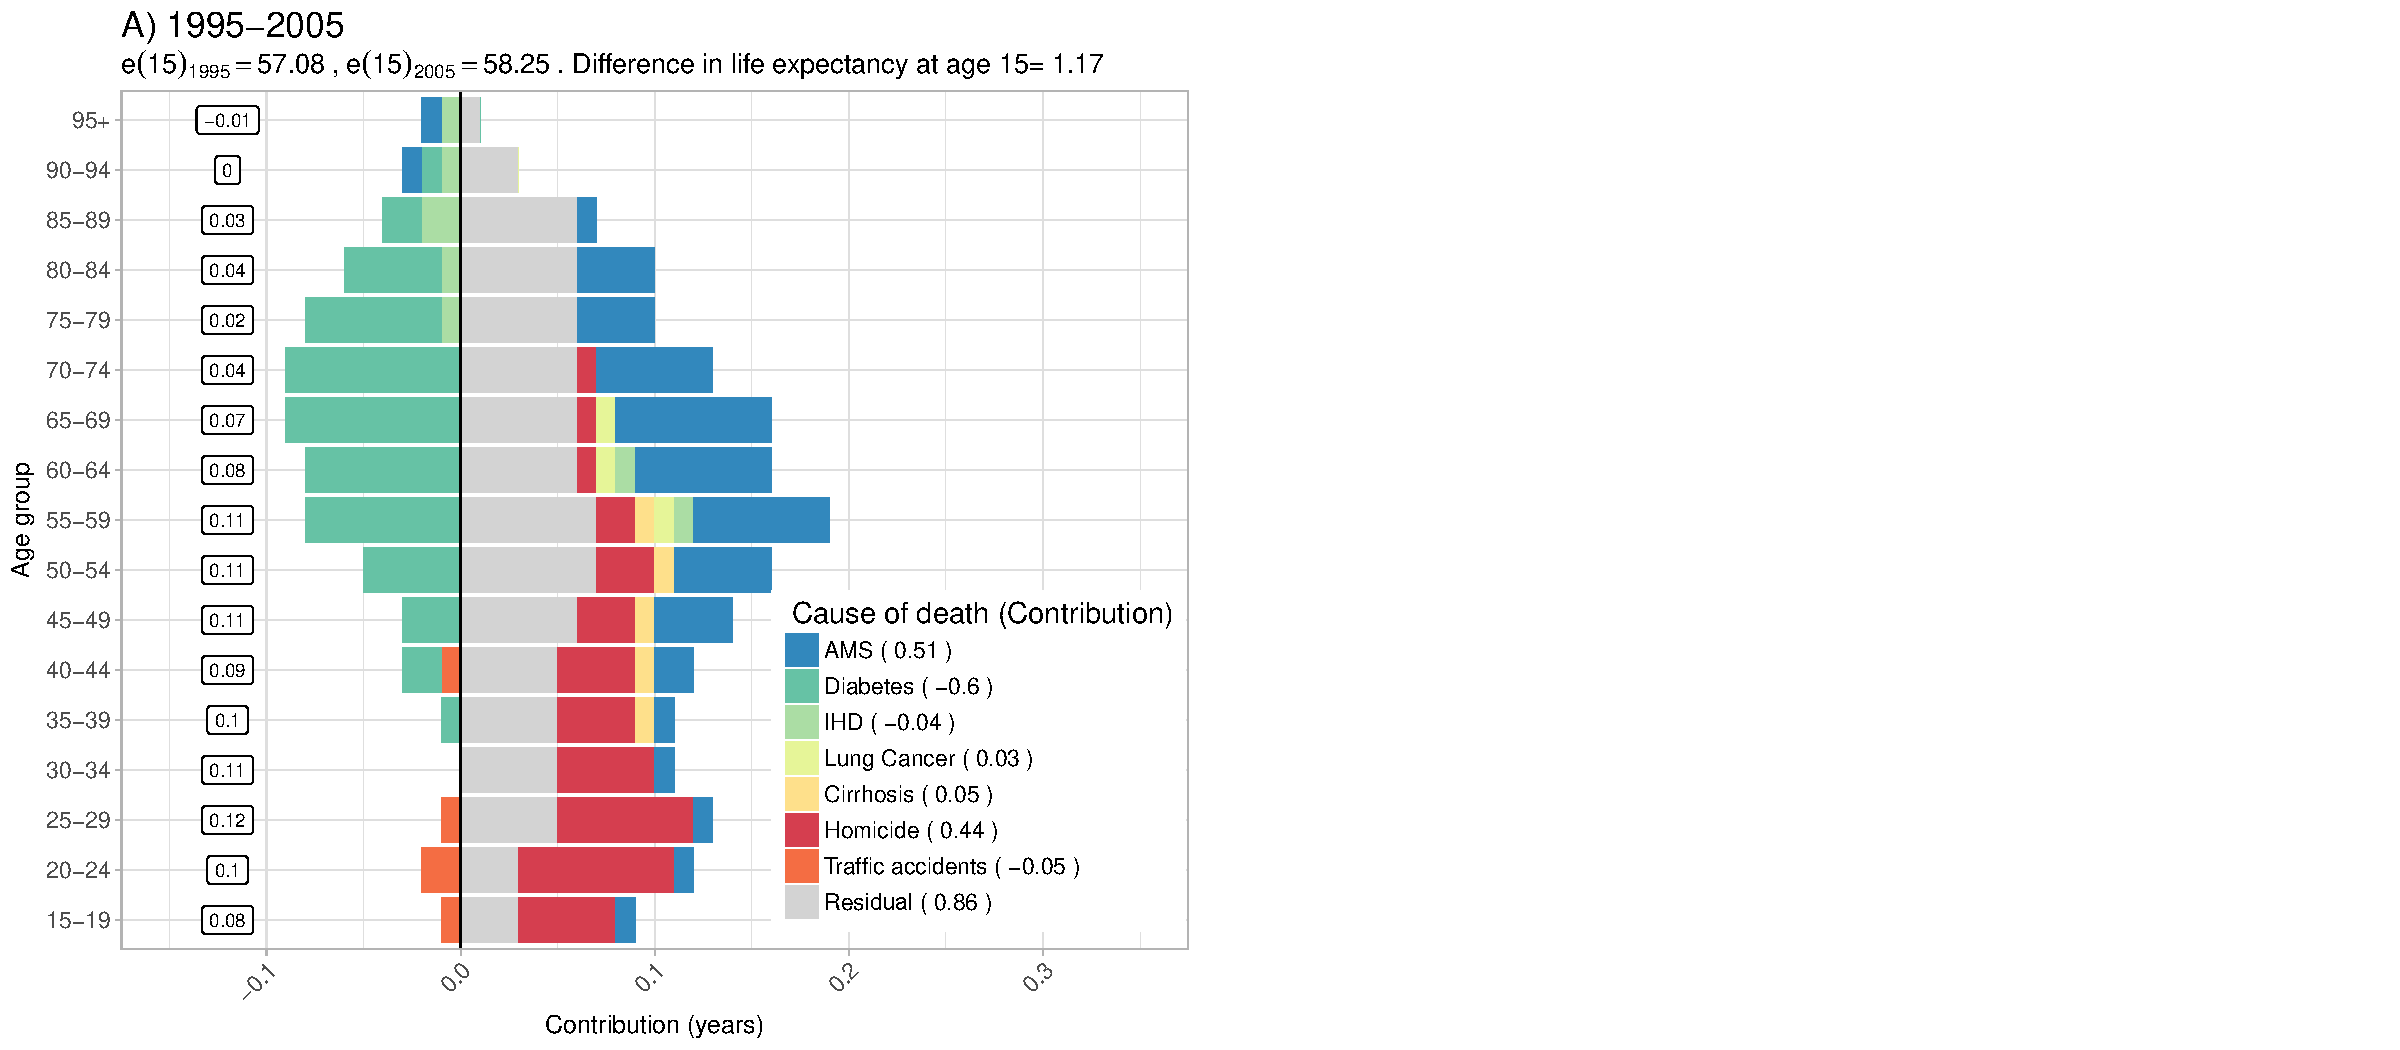
\includegraphics[scale=.31]{Figures/Figure_1_2}

\end{frame}


\begin{frame}
\begin{center}
\Large{\textbf{Esperanza de vida nacional}}
\end{center}

\hspace*{-1cm}   
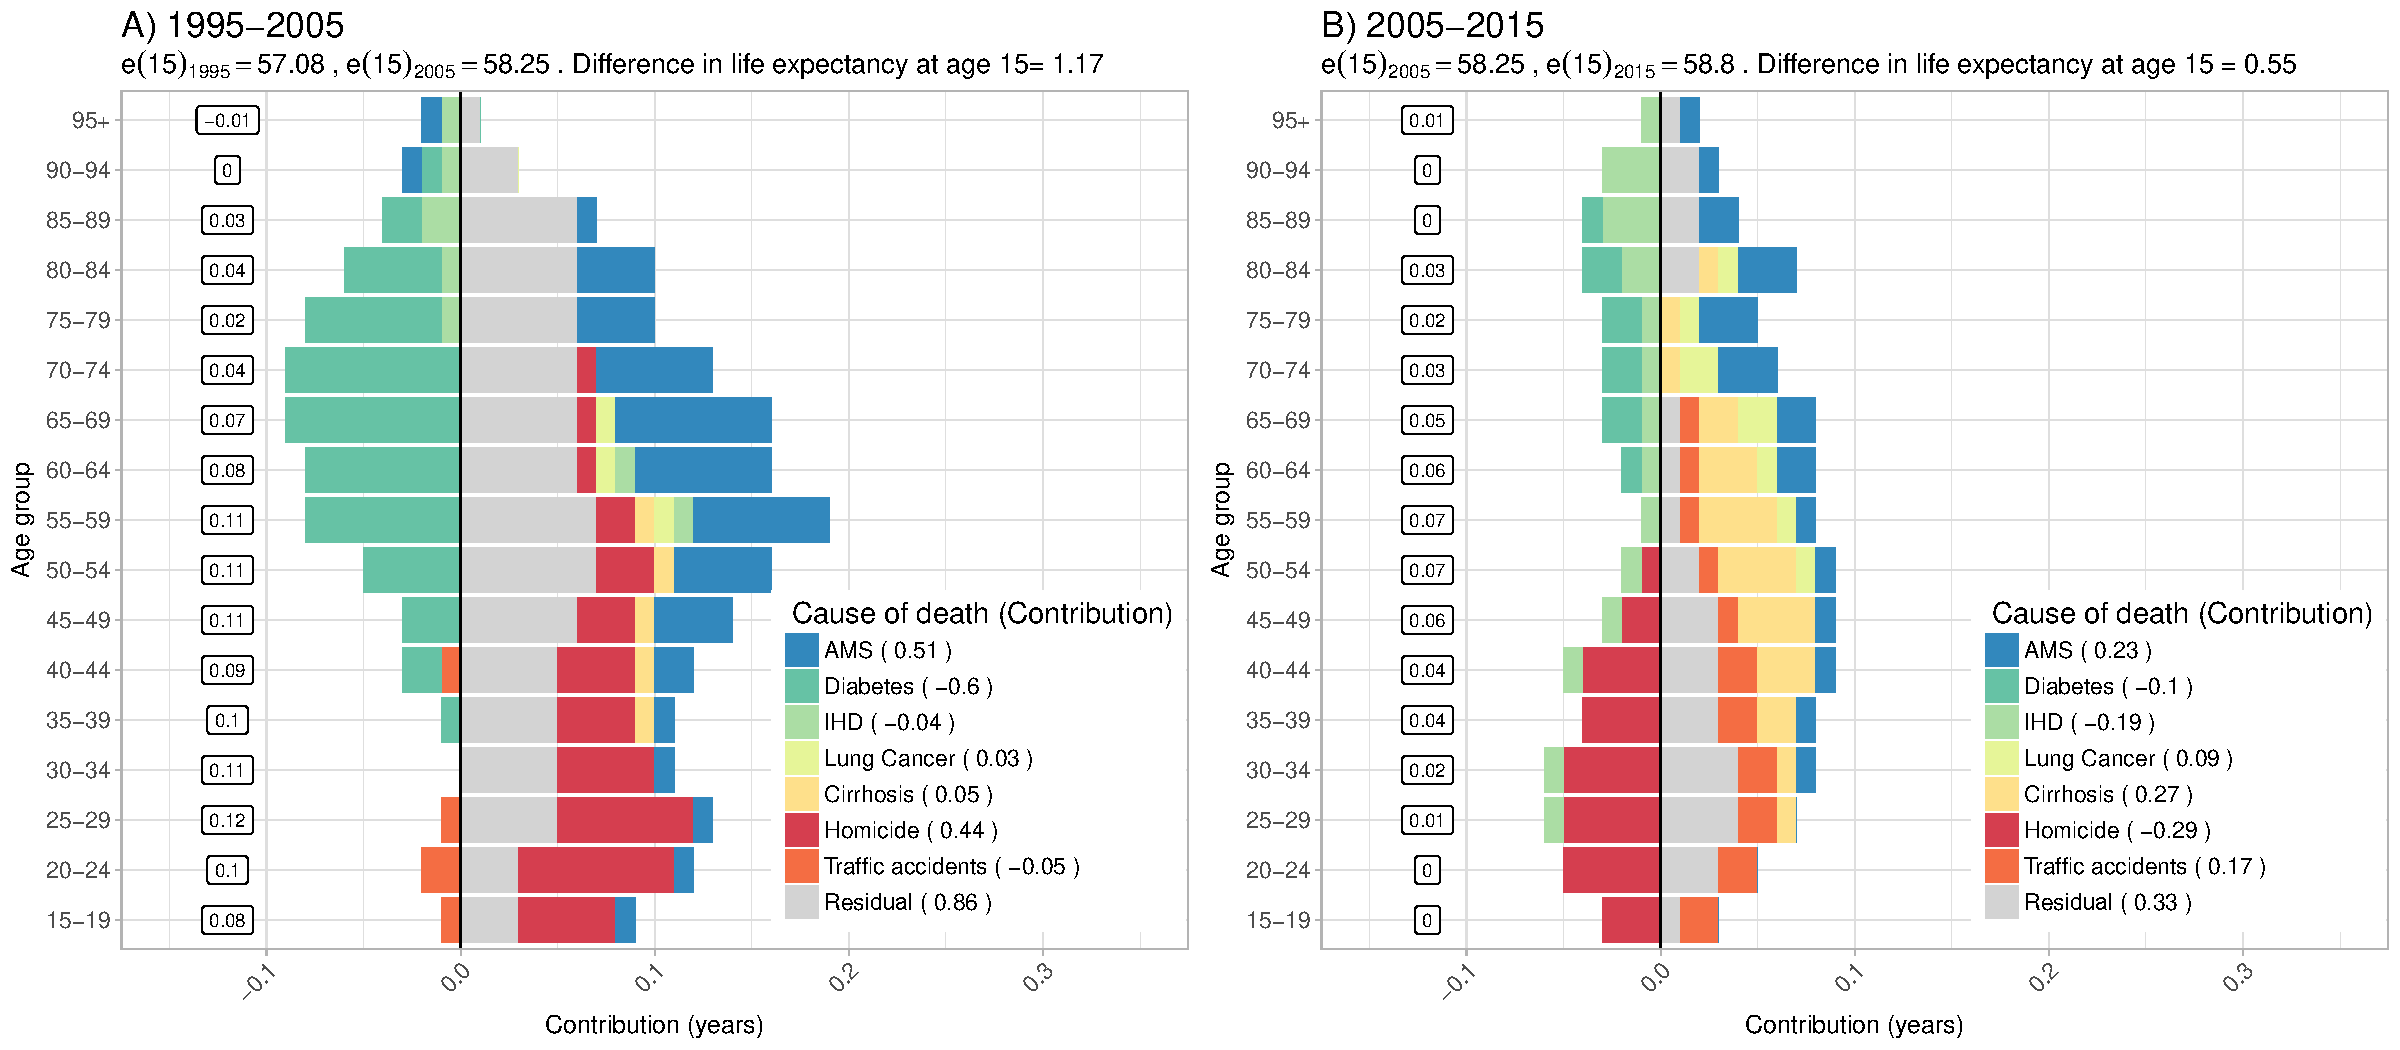
\includegraphics[scale=.31]{Figures/Figure_1}

\end{frame}


\begin{frame}
\begin{center}
\Large{\textbf{Disparidad en edad a la muerte }}
\end{center}

\hspace*{-1cm}   
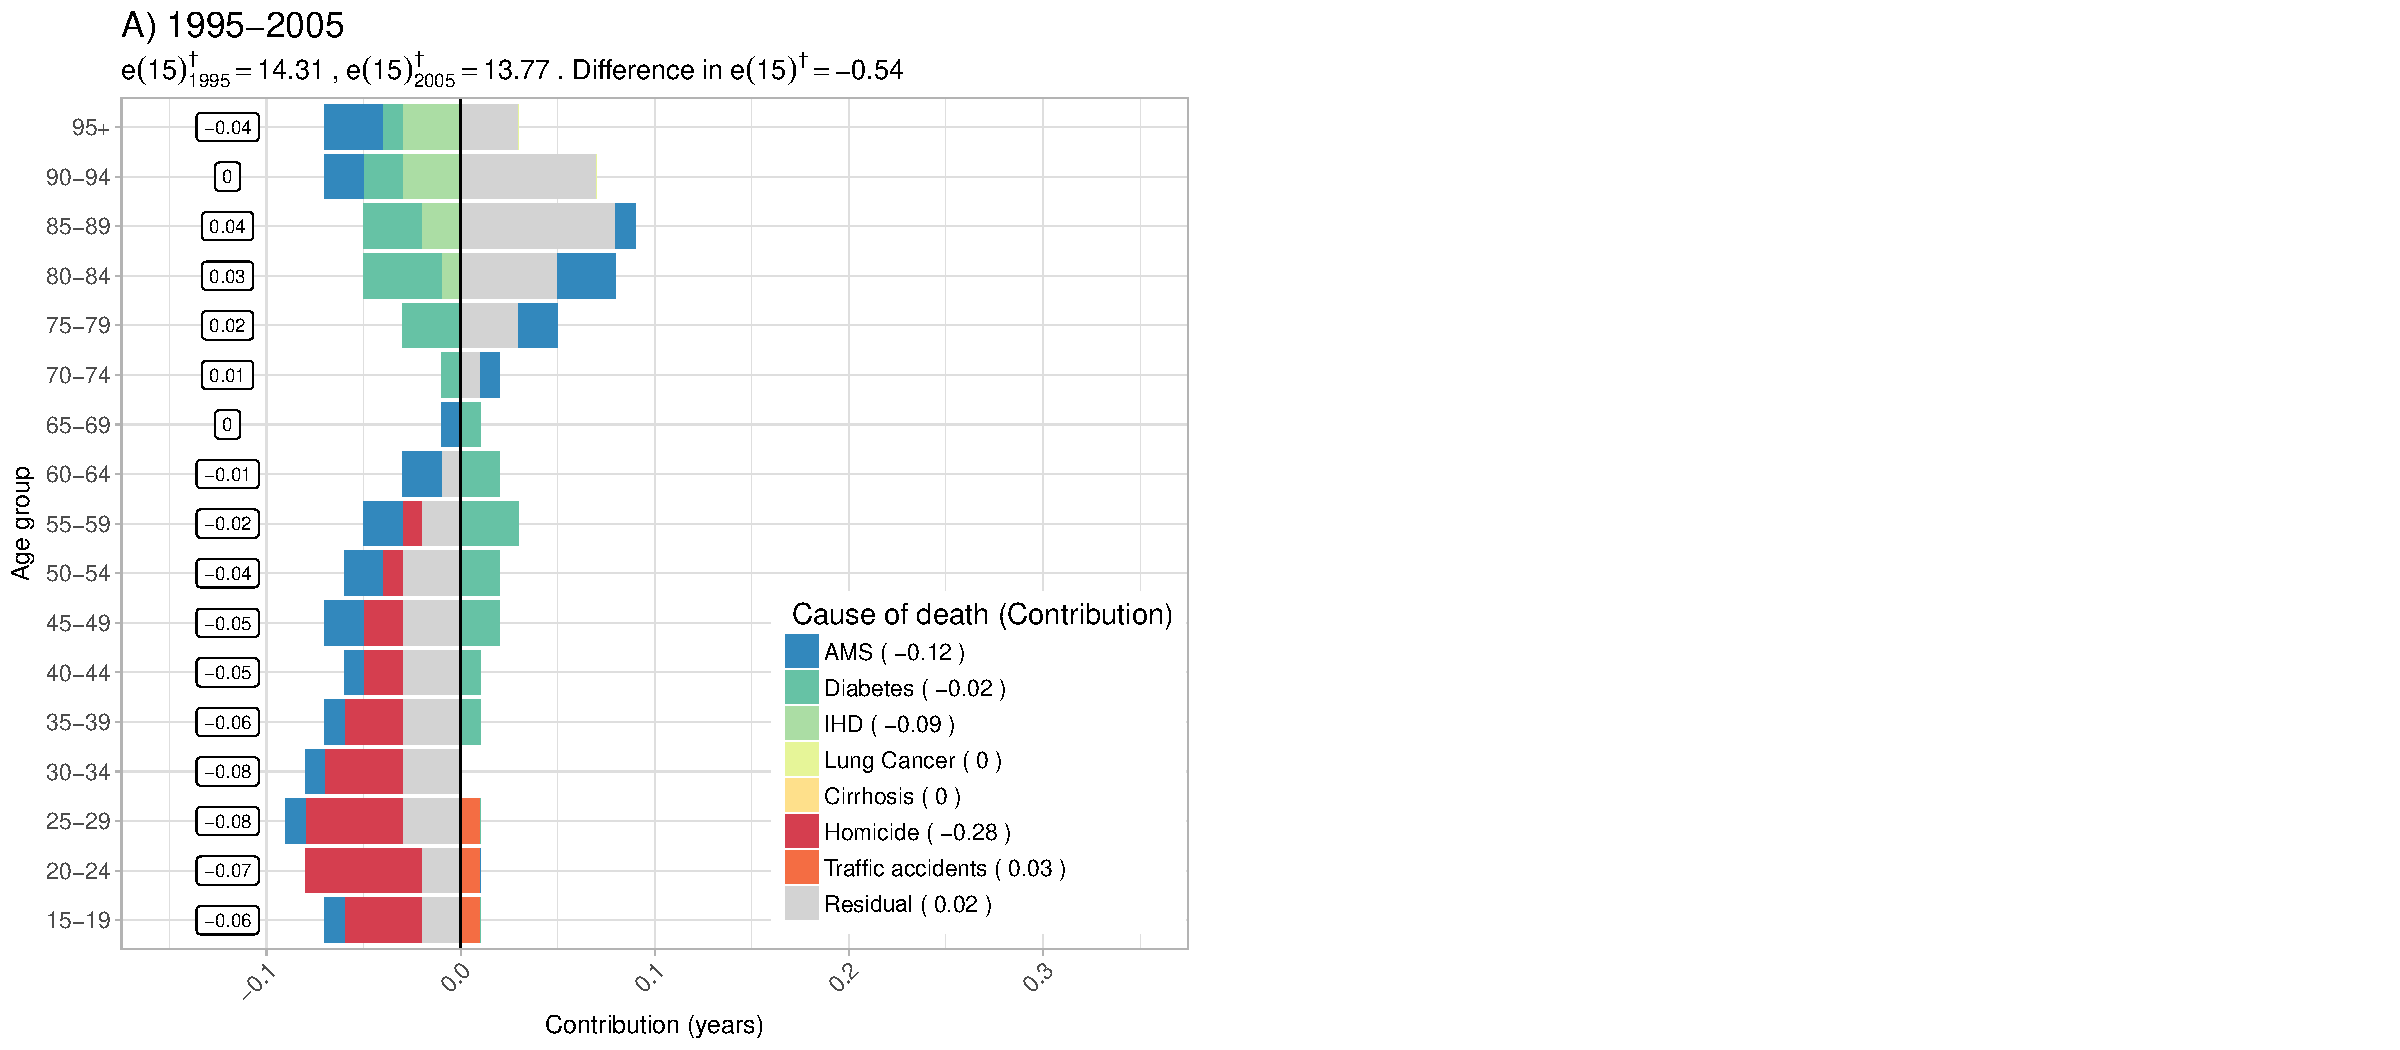
\includegraphics[scale=.31]{Figures/Figure_2_2}

\end{frame}


\begin{frame}
\begin{center}
\Large{\textbf{Disparidad en edad a la muerte}}
\end{center}

\hspace*{-1cm}   
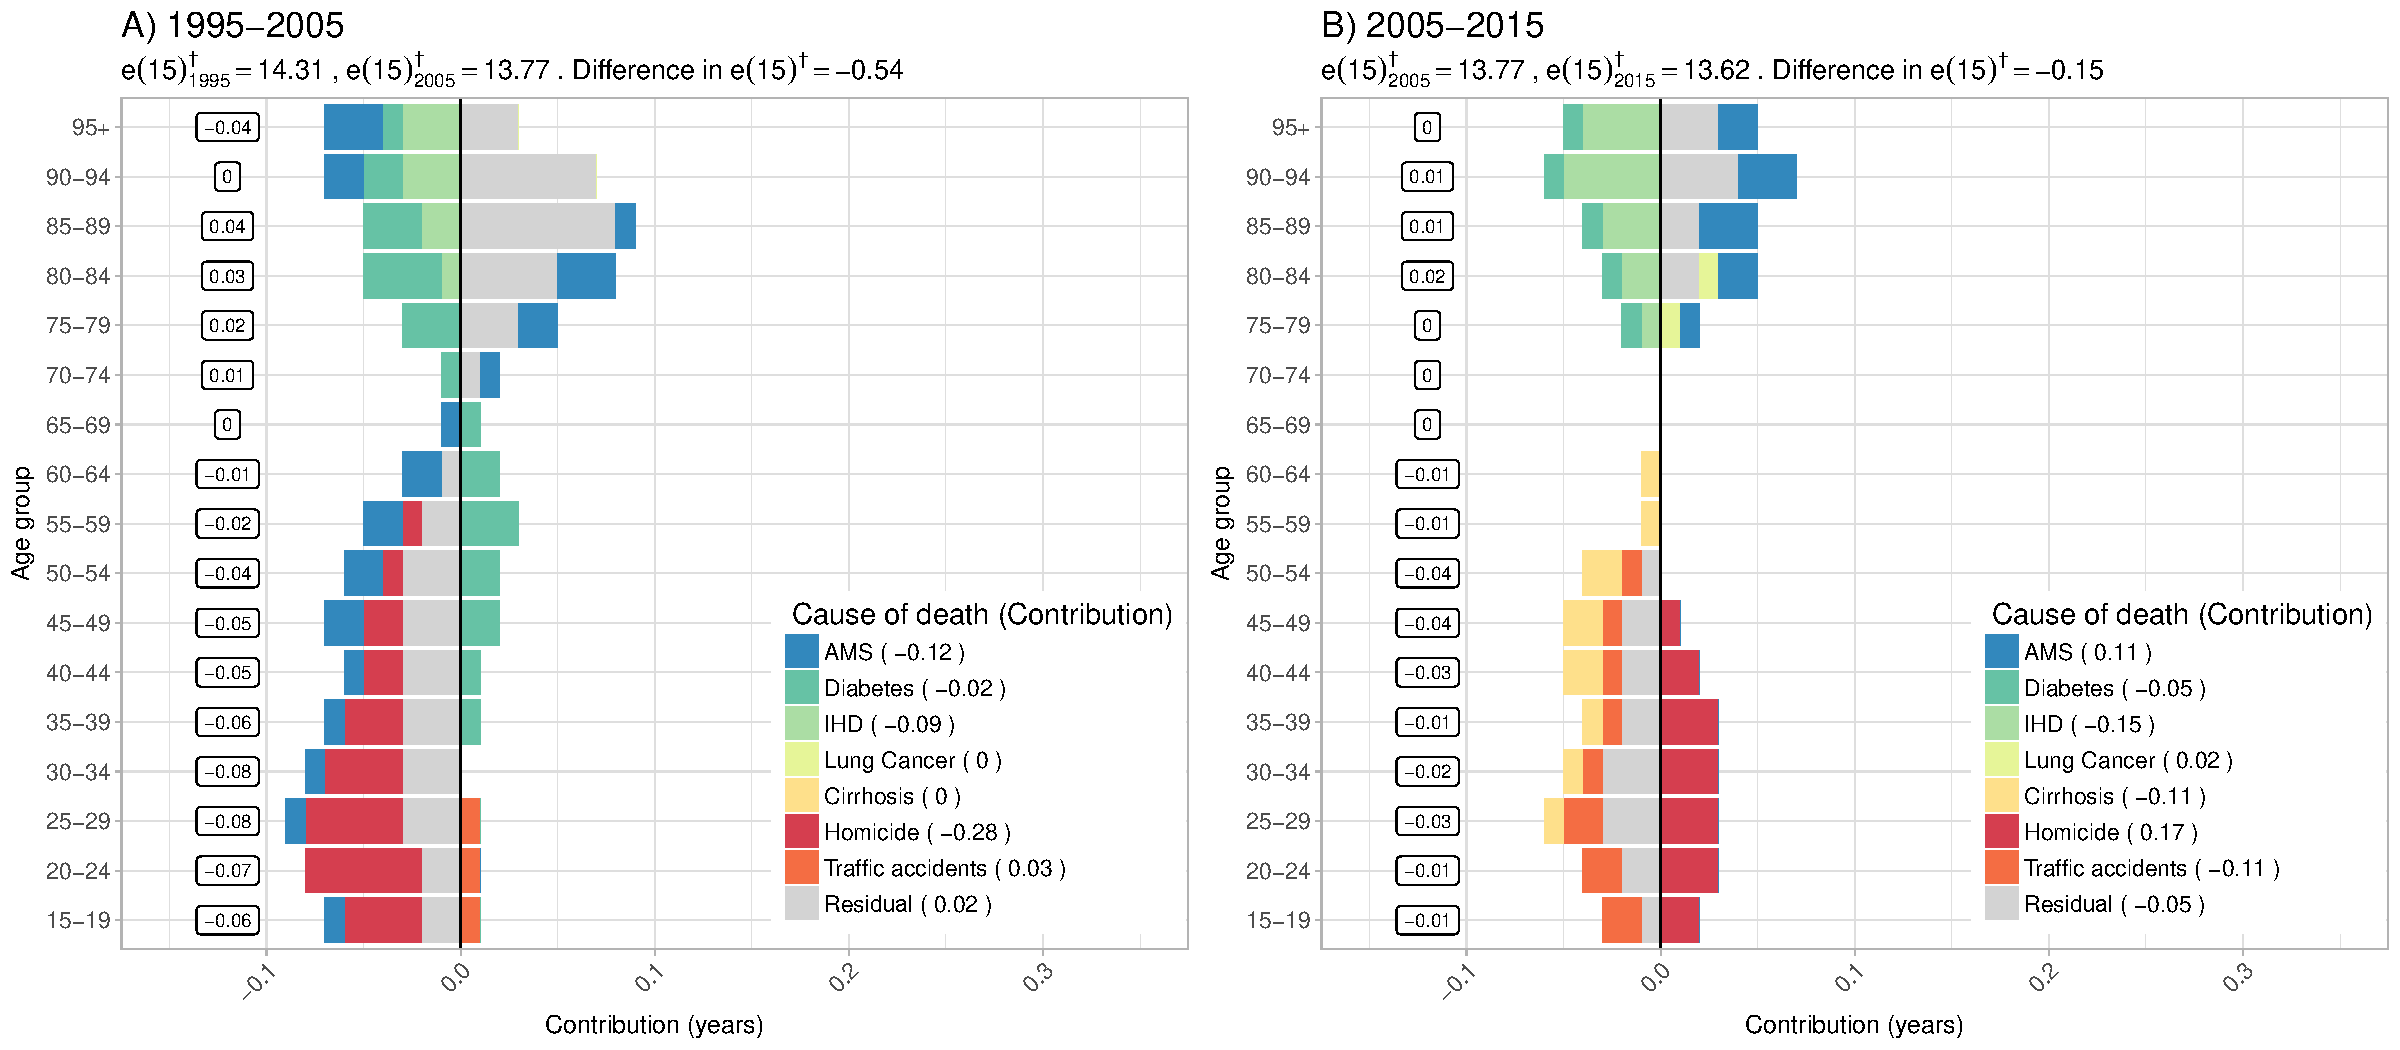
\includegraphics[scale=.31]{Figures/Figure_2}

\end{frame}


\begin{frame}
\begin{center}
\Large{\textbf{Nivel estatal}}
\end{center}

\hspace*{-1cm}   
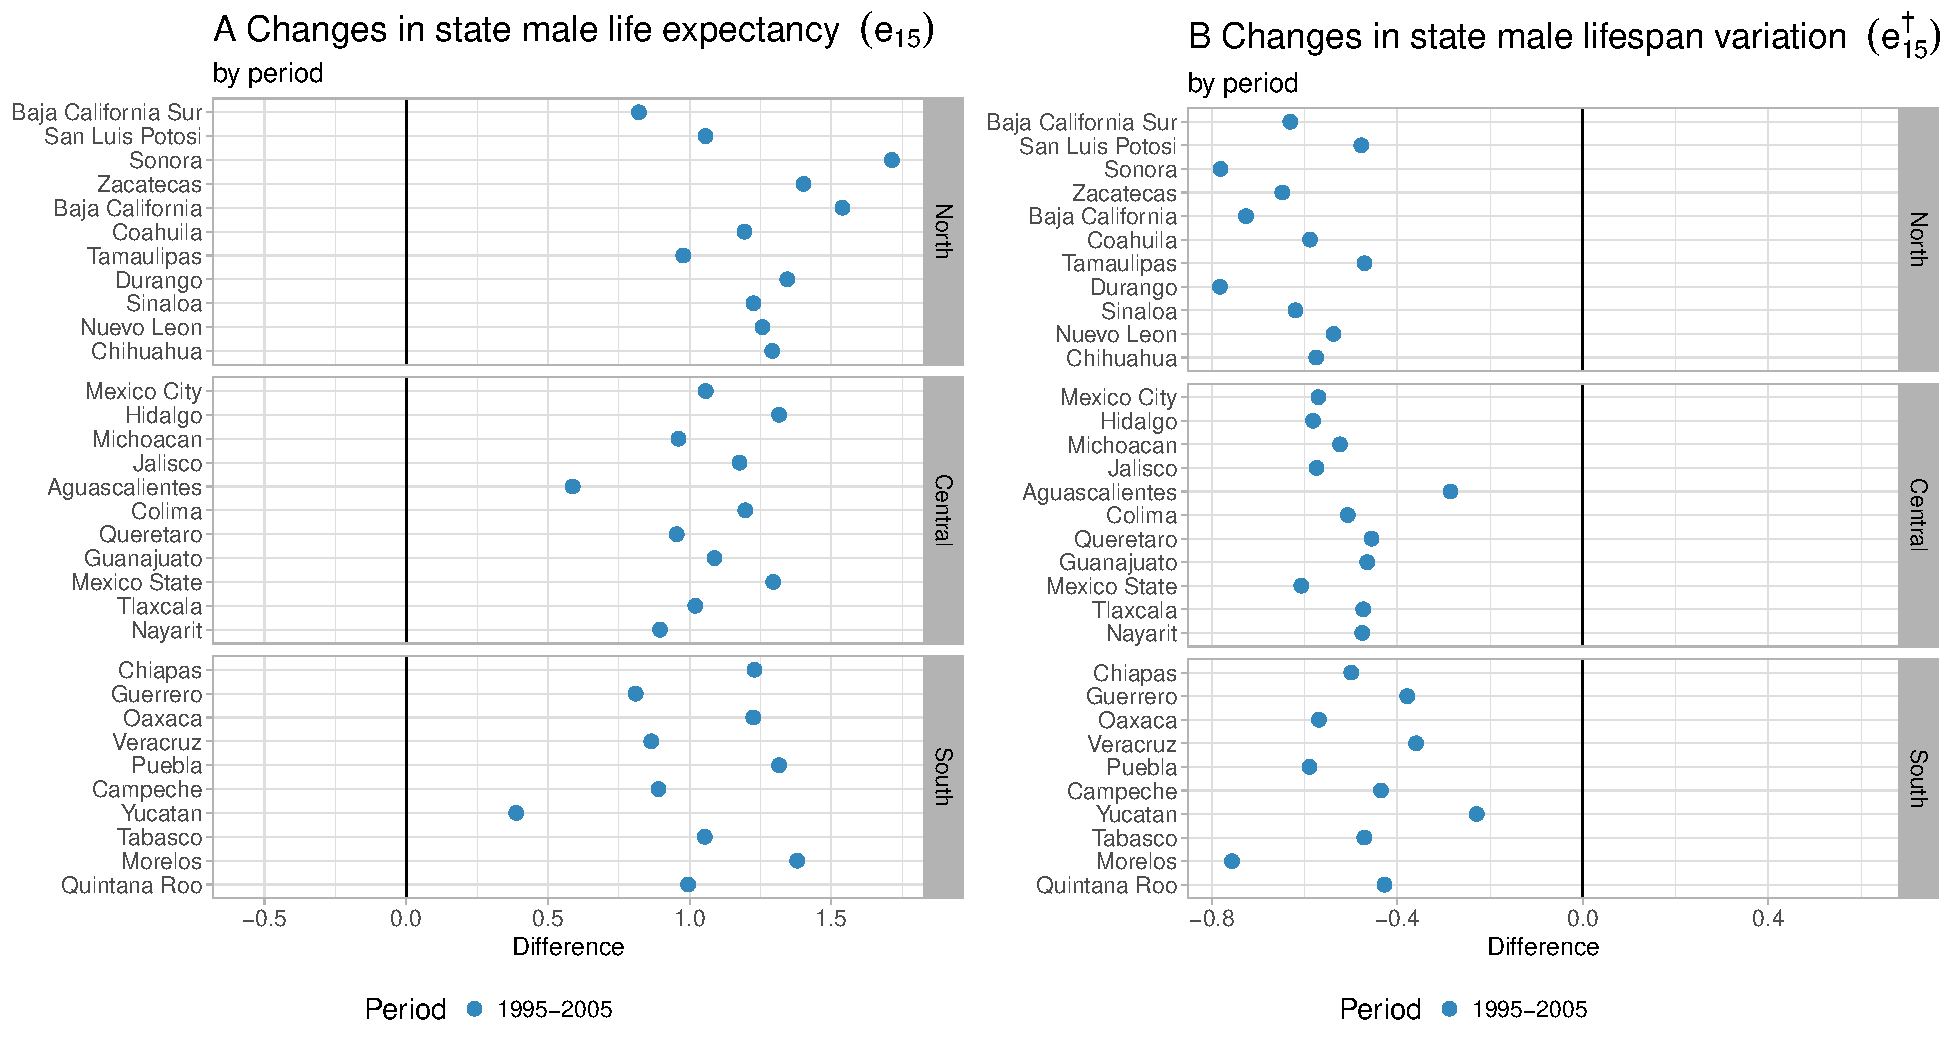
\includegraphics[scale=.38]{Figures/Figure_3_1}

\end{frame}


\begin{frame}
\begin{center}
\Large{\textbf{Nivel estatal}}
\end{center}

\hspace*{-1cm}   
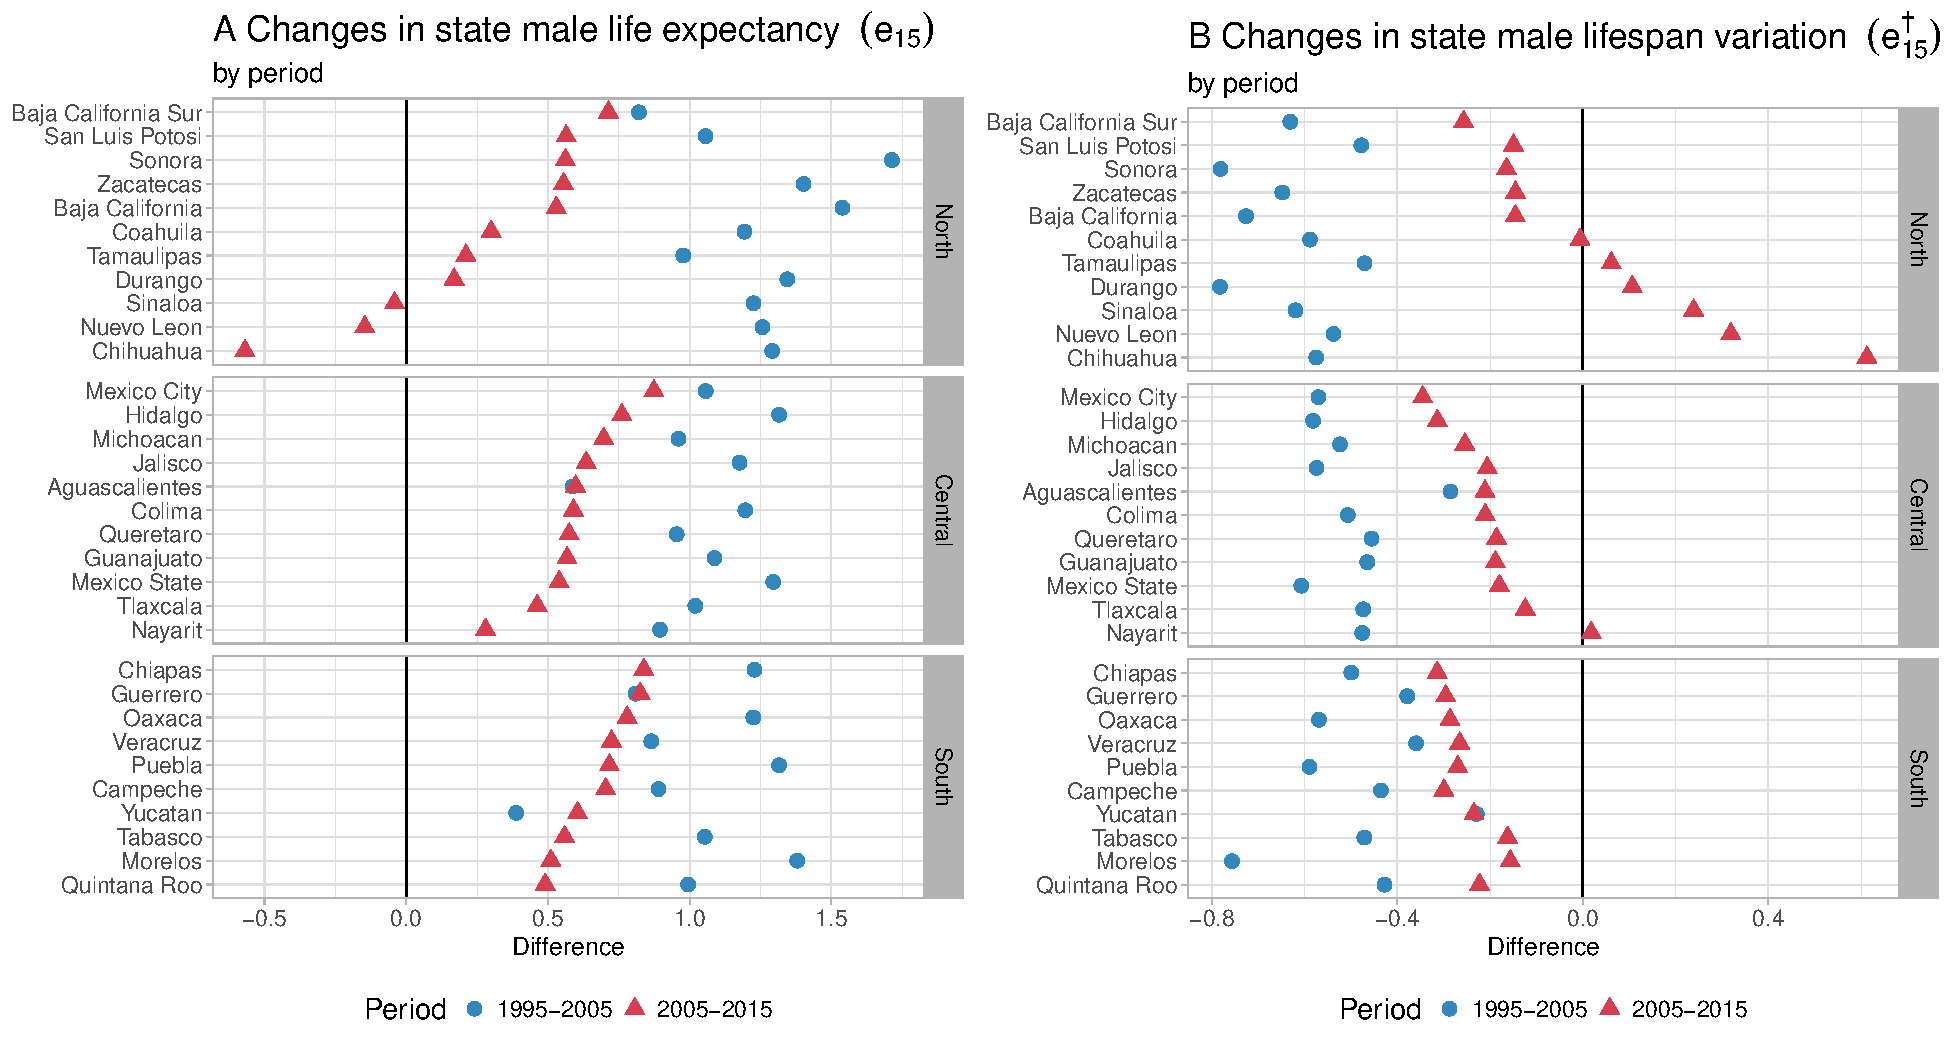
\includegraphics[scale=.38]{Figures/Figure_3}

\end{frame}



\begin{frame}

\Large{
Chihuahua: Tasas 3 veces las de tropas militares de USA en Iraq entre 2003 y 2006!
				\begin{center}
		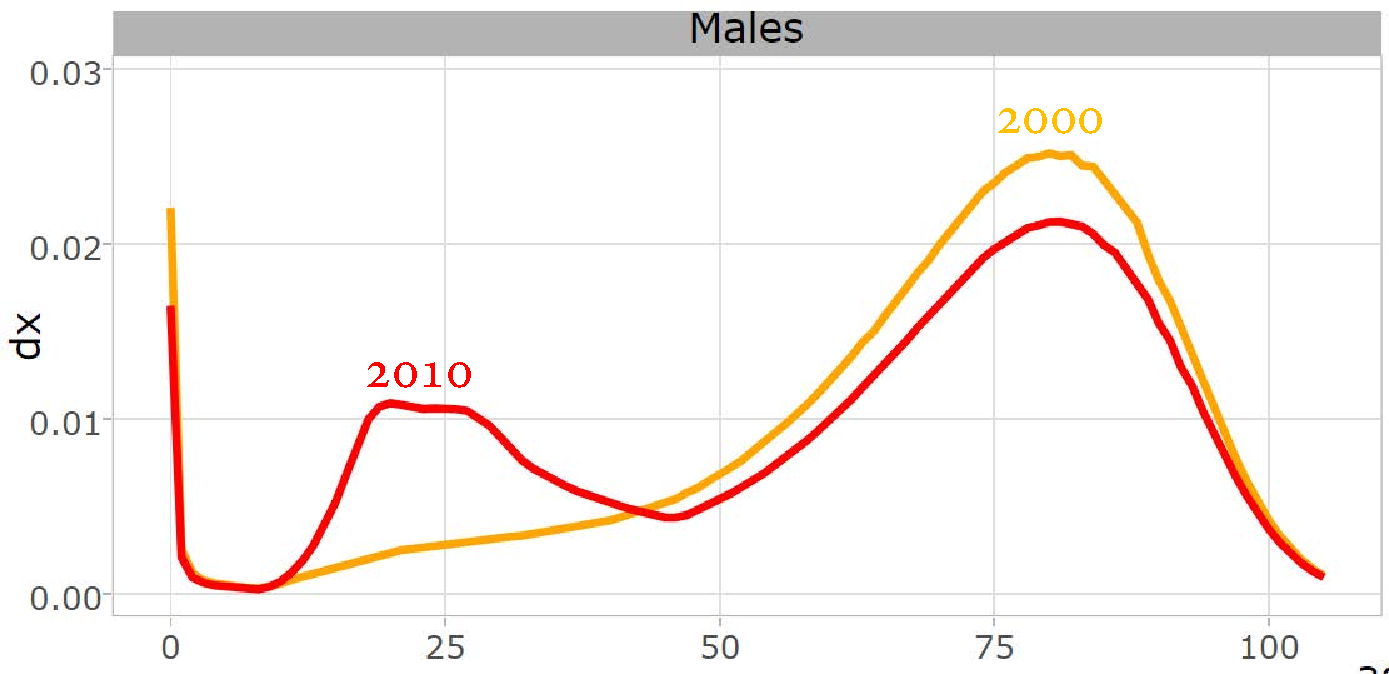
\includegraphics[scale=.45]{Figures/Distr_chihuahua}
				\end{center}				

}
\end{frame}



\begin{frame}
\begin{center}
\Large{\textbf{Causas de muerte}}
\end{center}

\hspace*{-1cm}   
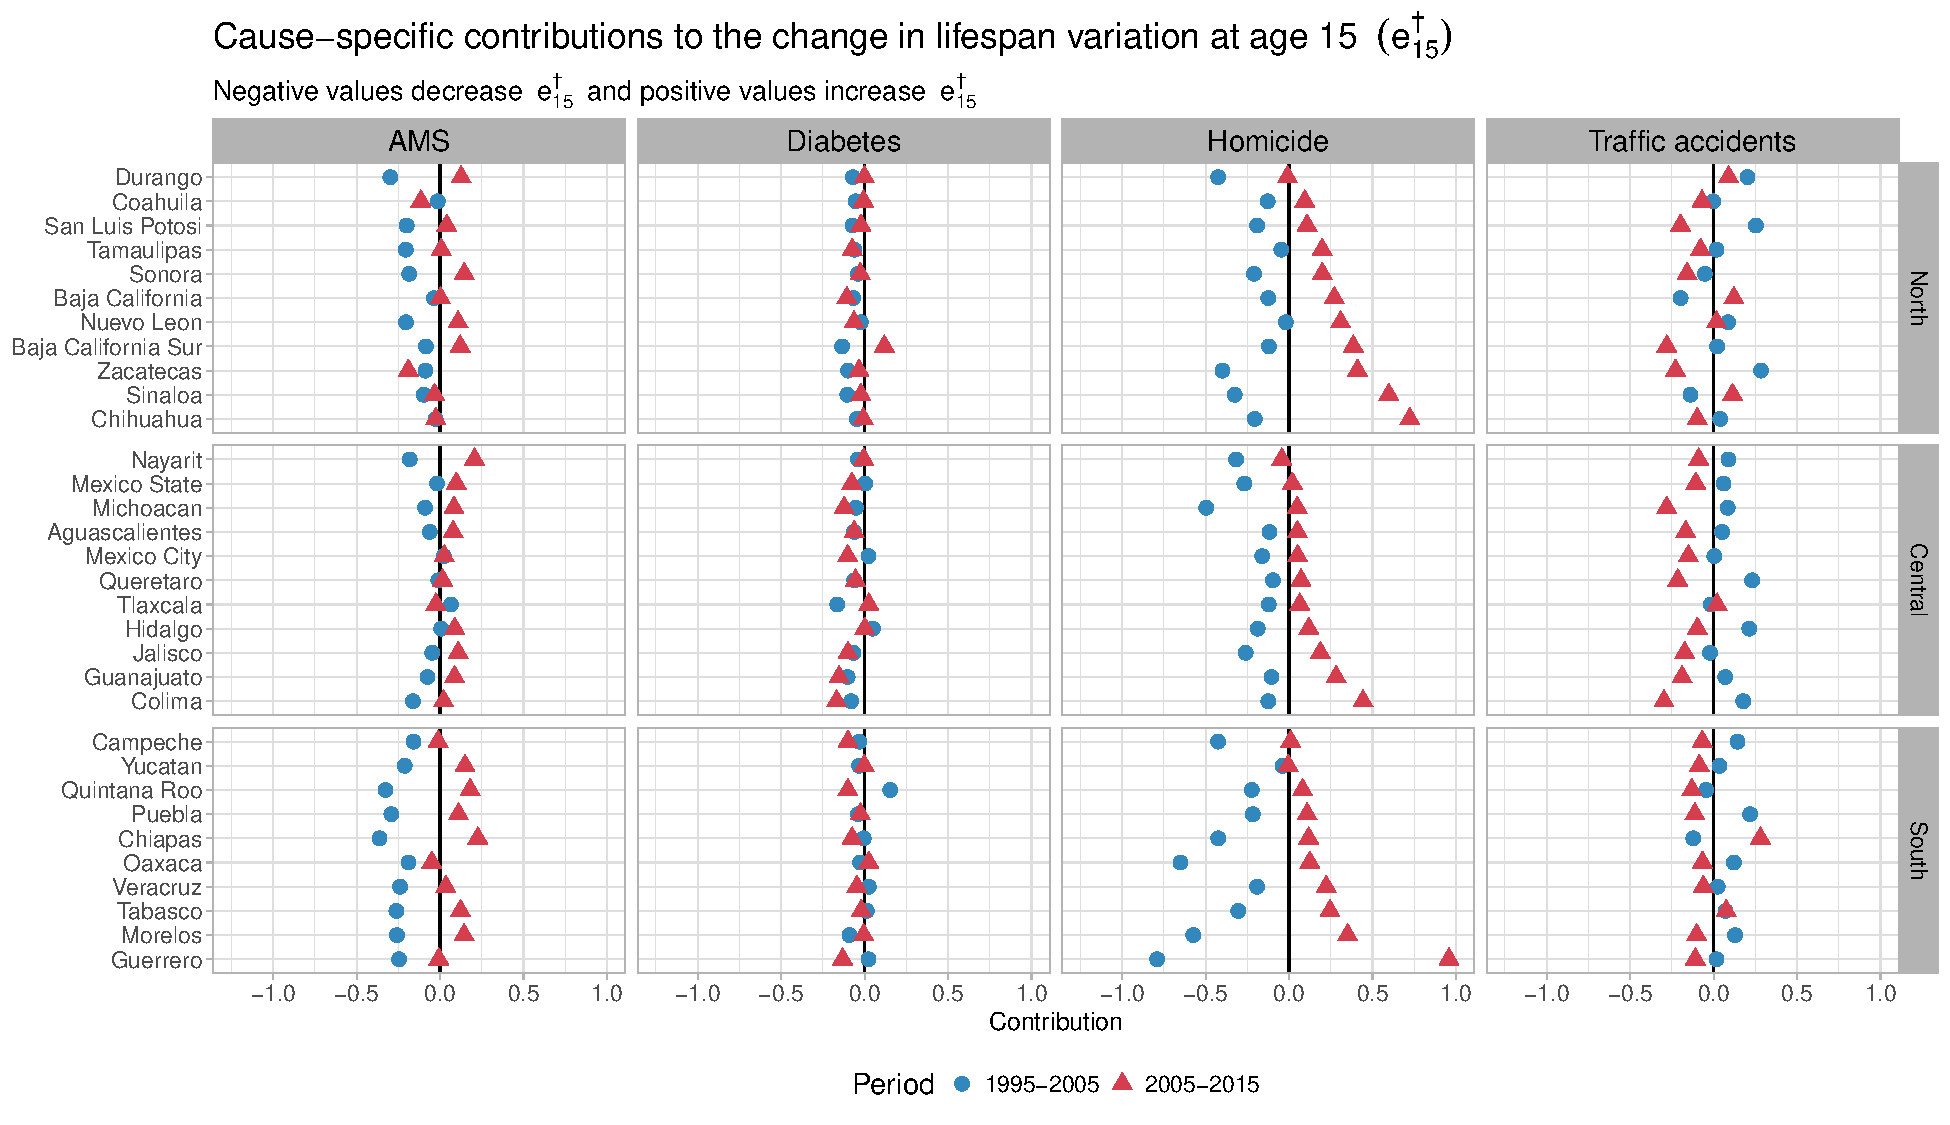
\includegraphics[scale=.38]{Figures/Figure_4}

\end{frame}


\begin{frame}

\Large{
2 de las ciudades m\'as peligrosas del mundo!

				\begin{center}
		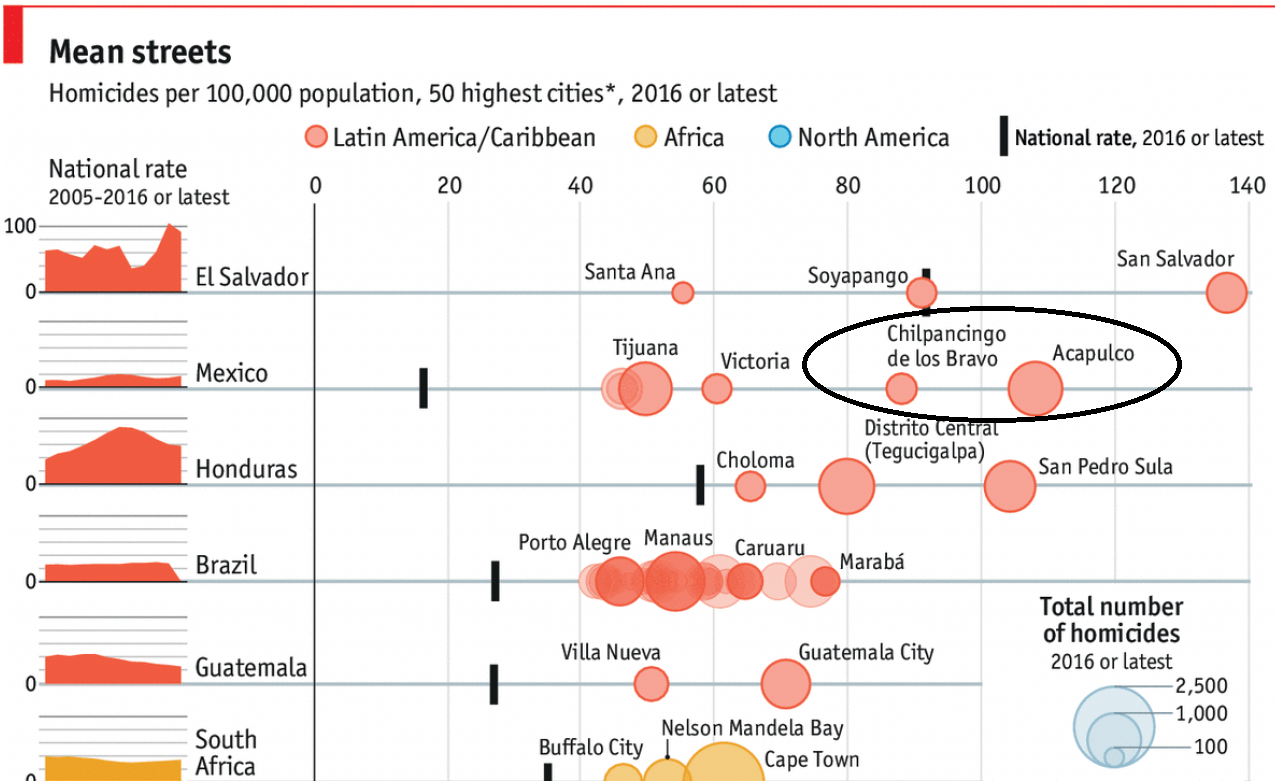
\includegraphics[scale=.38]{Figures/Capture}
				\end{center}				

}
\end{frame}


\begin{frame}
\Huge{
\begin{center}
Perspectiva internacional \linebreak \\

{\fontsize{70}{80}\selectfont 

 $\backsim$ 2,000,000}\\
15-30

\end{center}
}
\end{frame}

\begin{frame}
\Huge{
\begin{center}
{\fontsize{70}{80}\selectfont 77\%}\\
Hombres

\end{center}
}
\end{frame}


\begin{frame}
\Huge{
\begin{center}
{\fontsize{70}{80}\selectfont 35\% Homicidios}\\
(+ 1/2 million)

\end{center}
}
\end{frame}


\begin{frame}
\Large{
Conclusiones \pause

		\begin{itemize}
		
		\item Homicidios \textbf{revirtieron} ganancias en $e_0$ y aumentaron la disparidad. \pause

		\item \textbf{A 10y} de la guerra con las drogas, Mexico no ha sido capaz de regresar a los niveles de \textbf{2005}. \pause
		
		\item Hombre j\'ovenes viven menos y tienen mayor incertidumbre \pause
		
		\item \textbf{La violencia} en Mexico $\longrightarrow$ \textbf{prioridad urgente}. \pause
		
		\item Otros pa\'ises en AL podr\'ian experimentar similares efectos de homicidios.
						
		\end{itemize}

}
\end{frame}






%%%%%%%%%%%%%%%%%%%%%%%%%%%%%%%%%%%%%%%%%%%%%%%%%%%%%%%%%%%%%%%%%%%%%%%%

%%%%%%%%%%%%%%%%%%%%%%%%%%%%%%%%%%%%%%%%%%%%%%%%%%%%%%%%%%%%%%%%%%%%%%%%
\begin{frame}
 \begin{center}
	\begin{center}
	 \textbf{Reto de M\'exico: Reducir la violencia}
	\end{center}

	\bigskip

Email: jmaburto@health.sdu.dk 

\faTwitter \quad  @jm\_aburto 

\faGithub \quad @jmaburto 

Shinnyapp: \url{<https://demographs.shinyapps.io/LVMx_15_App/>}


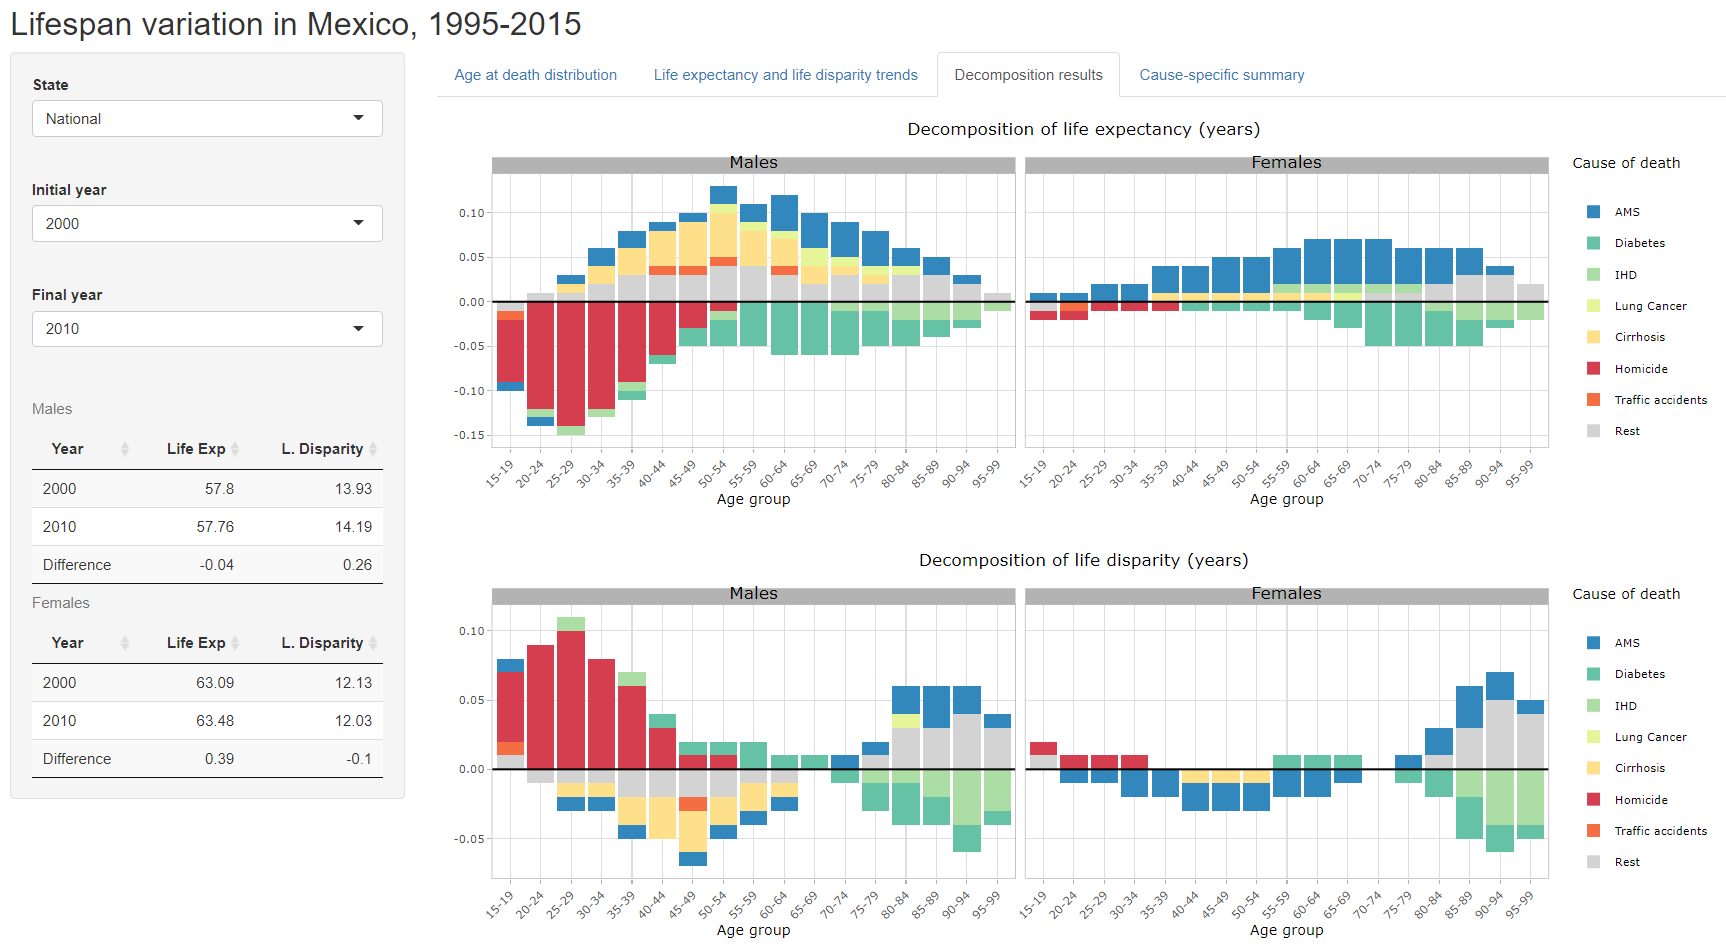
\includegraphics[scale=0.23]{Figures/Shinnyapp_fig} \\   

 

\end{center}
 
 

\end{frame}



\end{document}
	

